\documentclass[10pt,letterpaper]{article}
\usepackage[utf8]{inputenc}
\usepackage[T1]{fontenc}
\usepackage[spanish,es-noshorthands]{babel}
\usepackage[margin=2.2cm]{geometry}
\usepackage{amsmath,amssymb,mathtools}
\usepackage{graphicx}
\usepackage{booktabs}
\usepackage{enumitem}
\usepackage{caption}
\usepackage{lmodern}
\usepackage[expansion=false]{microtype}
\usepackage[hidelinks]{hyperref}
\setlist{nosep,leftmargin=1.2em}
\captionsetup{font=footnotesize,skip=2pt}
\setlength{\parskip}{2pt}
\setlength{\parindent}{0pt}
\usepackage{titlesec}
\titlespacing*{\section}{0pt}{6pt}{2pt}
\titlespacing*{\subsection}{0pt}{4pt}{1pt}
\titleformat{\section}{\large\bfseries}{\thesection.}{0.4em}{}
\titleformat{\subsection}{\normalsize\bfseries}{\thesubsection}{0.4em}{}
\newcommand{\dk}{d_k}

\begin{document}

\begin{center}
{\large\bfseries CC3092 -- Deep Learning y Sistemas Inteligentes}\\
{\large\bfseries Hoja de trabajo \#2: Transformers y mecanismos de atención}\\[2pt]
Angel Esquit \quad|\quad Repositorio: \url{https://github.com/AngelEsquit/HT2-DL}
\end{center}

\section{Investigación: de las RNN a la atención}
\textbf{Cuello de botella.} En un seq2seq con RNN el encoder comprime toda la oración fuente en un único vector de tamaño fijo (el último estado oculto), del que el decoder debe reconstruir la traducción. Cuanto más larga es la oración, más información debe caber en el mismo vector y el contenido temprano se diluye, por lo que la calidad cae con la longitud. Bahdanau et al.\ lo resuelven conservando todos los estados del encoder $h_1,\dots,h_n$ y, en cada paso del decoder, calculando una suma ponderada $c_t=\sum_i \alpha_{ti}h_i$ con $\alpha_{t\cdot}=\mathrm{softmax}(e_{t\cdot})$: el decoder «mira» las posiciones relevantes en vez de depender de un resumen único.

\textbf{Aditiva vs.\ multiplicativa.} Bahdanau usa $e_{ti}=v^\top\tanh(W_s s_{t-1}+W_h h_i)$, una pequeña red feed-forward por par; Luong usa $e_{ti}=s_t^\top h_i$ (o con una matriz intermedia). El producto punto se reduce a una multiplicación de matrices ($QK^\top$), operación sumamente optimizada en GPU/TPU, y no necesita materializar tensores intermedios por cada par ni parámetros extra, por lo que es más rápido y eficiente en memoria; para $d_k$ grande la versión aditiva rinde algo mejor si no se escala, motivo del factor $1/\sqrt{d_k}$.

\textbf{Query/key/value.} Es una búsqueda «suave» en un diccionario: la \emph{query} describe lo que se busca, cada \emph{key} lo que ofrece cada entrada y el \emph{value} es el contenido que se devuelve; en lugar de elegir la llave que coincide exactamente, se devuelve un promedio de valores ponderado por la similitud query--key (softmax). En \emph{self-attention} Q, K y V se obtienen de la misma secuencia $X$ mediante proyecciones lineales $XW^Q, XW^K, XW^V$; en \emph{cross-attention} Q viene del decoder y K, V de la salida del encoder.

\textbf{Limitaciones de la RNN que elimina el Transformer.} (i) Procesamiento secuencial: el estado $t$ depende del $t-1$, así que no se paraleliza a lo largo de la secuencia; la self-attention procesa todas las posiciones a la vez. (ii) Dependencias largas: la información entre dos tokens a distancia $d$ atraviesa $O(d)$ pasos recurrentes, mientras que en atención la longitud del camino es $O(1)$. (iii) Desvanecimiento/explosión del gradiente: al retropropagar por $d$ pasos el gradiente es un producto de $d$ jacobianos; con el camino directo de la atención (y las conexiones residuales) esto se mitiga.

\section{Investigación: la arquitectura Transformer}
\textbf{Scaled dot-product attention:} $\mathrm{Attn}(Q,K,V)=\mathrm{softmax}(QK^\top/\sqrt{\dk})V$ produce, para cada query, un promedio de los valores ponderado por su afinidad con las llaves. Si las componentes de $q,k$ son independientes con media 0 y varianza 1, cada término $q_ik_i$ tiene media 0 y varianza 1, y como son independientes $\mathrm{Var}(q\cdot k)=\dk$. Con $\dk$ grande los puntajes tienen desviación $\sqrt{\dk}$, el softmax se satura (una probabilidad $\approx1$, el resto $\approx0$) y su gradiente $\partial p_i/\partial s_j=p_i(\delta_{ij}-p_j)$ se anula, frenando el aprendizaje. Dividir entre $\sqrt{\dk}$ devuelve la varianza a 1 (verificado en \S\ref{sec:verif}).

\textbf{Multi-head attention:} con $h$ cabezas de dimensión $d_{model}/h$ el modelo atiende a distintas posiciones y «subespacios de representación» a la vez (una sola cabeza promedia todo en un único patrón). El número de parámetros \emph{no cambia}: $W^Q,W^K,W^V$ son $d_{model}\times d_{model}$ en total y $W^O$ también, $4d_{model}^2$ (+sesgos) con cualquier $h$; el costo de cómputo tampoco cambia sustancialmente.

\textbf{Codificación posicional:} la atención es equivariante a permutaciones (sin posiciones, «perro muerde hombre» y «hombre muerde perro» dan lo mismo), así que se inyecta el orden. La versión sinusoidal suma a cada embedding $PE_{(pos,2i)}=\sin(pos/10000^{2i/d})$, $PE_{(pos,2i+1)}=\cos(\cdot)$: es determinista, no añade parámetros y $PE_{pos+k}$ es función lineal de $PE_{pos}$, lo que facilita atender a desplazamientos relativos. Los embeddings aprendidos son una tabla entrenable (rinden similar, pero limitados a la longitud máxima vista). RoPE rota $q$ y $k$ en cada par de dimensiones un ángulo proporcional a la posición, de modo que $q_m\!\cdot k_n$ depende solo de $m-n$ (posición relativa) y extrapola mejor; es el usual en modelos recientes.

\textbf{Bloque completo:} cada subcapa (atención y FFN por posición, $\mathrm{ReLU}(xW_1)W_2$, que aporta no linealidad y capacidad por token) va envuelta en una conexión residual, que facilita el flujo de gradiente en redes profundas, y en LayerNorm, que estabiliza las activaciones. Post-LN (original) calcula $\mathrm{LN}(x+\mathrm{Sub}(x))$; Pre-LN calcula $x+\mathrm{Sub}(\mathrm{LN}(x))$, dejando un camino residual sin normalizar. Pre-LN entrena de forma más estable y tolera mayor tasa de aprendizaje y menos \emph{warm-up}; Post-LN puede dar algo más de calidad pero es más difícil de entrenar a gran profundidad.

\textbf{Complejidad:} la self-attention cuesta $O(n^2d)$ en tiempo y $O(n^2)$ en memoria por la matriz $n\times n$ (frente a $O(nd^2)$ de una RNN, pero con profundidad secuencial $O(1)$). Propuestas: \emph{FlashAttention} calcula la misma atención exacta por bloques en SRAM sin materializar la matriz (memoria lineal, menos accesos a HBM; sigue siendo $O(n^2)$ en cómputo); atención por ventanas/dispersa (Longformer) limita cada token a una vecindad más tokens globales ($O(nw)$), sacrificando interacciones directas de largo alcance; atención lineal (kernels, Performer) aproxima el softmax y logra $O(n)$, sacrificando precisión/expresividad (atención «nítida»).

\section{Investigación: atención en PyTorch y Hugging Face}
\begin{itemize}
\item \texttt{F.scaled\_dot\_product\_attention(q,k,v,attn\_mask,dropout\_p,is\_causal,scale)}: implementa la fórmula anterior con kernels fusionados (FlashAttention cuando es posible). \texttt{attn\_mask}: booleana (\texttt{True} = \emph{puede} atender) o flotante aditiva; \texttt{dropout\_p}: dropout sobre los pesos; \texttt{is\_causal}: aplica máscara triangular (no se combina con \texttt{attn\_mask}); \texttt{scale}: reemplaza el $1/\sqrt{\dk}$ por defecto.
\item \texttt{nn.MultiheadAttention(embed\_dim,num\_heads,batch\_first,kdim,vdim)}: proyecta, divide en cabezas, aplica atención y proyecta de salida; \texttt{kdim/vdim} permiten llaves/valores de otra dimensión (cross-attention). En \texttt{forward}: \texttt{key\_padding\_mask} (\texttt{(B,S)}, ignora tokens de relleno), \texttt{attn\_mask} (\texttt{(L,S)} o \texttt{(B·h,L,S)}; ojo: con máscara booleana \texttt{True} significa \emph{bloqueado}, al revés que en SDPA), \texttt{need\_weights} (devolver o no los pesos) y \texttt{average\_attn\_weights} (promediar cabezas o devolver \texttt{(B,h,L,S)}).
\item \texttt{nn.TransformerEncoderLayer(d\_model,nhead,dim\_feedforward,dropout,norm\_first)}: self-attention + FFN con residuales y LayerNorm; \texttt{norm\_first=True} da Pre-LN (por defecto Post-LN). \texttt{nn.Transformer.}\allowbreak\texttt{generate\_square\_}\allowbreak\texttt{subsequent\_mask(sz)} devuelve una matriz \texttt{sz×sz} con $-\infty$ sobre la diagonal y 0 en el resto (máscara causal aditiva).
\item Hugging Face: con \texttt{output\_attentions=True} (y \texttt{attn\_implementation="eager"}, pues SDPA/Flash no devuelven pesos) el modelo retorna una tupla con un tensor por capa de forma $(\text{batch},\text{cabezas},n,n)$; cada fila ya está normalizada con softmax.
\end{itemize}

\section{Ejercicio a mano y verificaciones}\label{sec:verif}
\textbf{Ejercicio a mano} ($n=3$, $\dk=2$). $Q=K=\begin{psmallmatrix}1&0\\0&1\\1&1\end{psmallmatrix}$, $V=\begin{psmallmatrix}1&2\\3&4\\5&6\end{psmallmatrix}$. Se calcula $QK^\top=\begin{psmallmatrix}1&0&1\\0&1&1\\1&1&2\end{psmallmatrix}$ y se divide entre $\sqrt2$ (entradas $0.707$, $0$, $1.414$). Fila 1: $e^{0.707}=2.028$, $e^0=1$, suma $5.056$, pesos $(0.401,0.198,0.401)$, salida $0.401(1,2)+0.198(3,4)+0.401(5,6)=(3.00,4.00)$. Fila 2: $(0.198,0.401,0.401)\Rightarrow(3.41,4.41)$. Fila 3: $e^{1.414}=4.113$, suma $8.169$, pesos $(0.248,0.248,0.503)\Rightarrow(3.51,4.51)$. La implementación desde cero y \texttt{F.scaled\_dot\_product\_attention} coinciden con estos valores (\texttt{allclose}).

\textbf{Verificaciones.} (a) Con $q,k\sim\mathcal N(0,I)$ ($2\times10^4$ muestras), $\mathrm{Var}(q\cdot k)=3.98,\,16.07,\,64.25,\,253.1,\,1015.6$ para $\dk=4,16,64,256,1024$ (teoría: $\dk$), y tras dividir por $\sqrt{\dk}$ queda $\approx1.00$. (b) Con 16 llaves, la probabilidad máxima sin escalar sube de $0.43$ ($\dk=4$) a $0.96$ ($\dk=1024$) y la norma del gradiente cae de $4.9\!\times\!10^{-2}$ a $5.1\!\times\!10^{-3}$; con escalamiento permanecen en $\approx0.24$ y $\approx5.8\!\times\!10^{-2}$ (Fig.~\ref{fig:esc}). (c) \texttt{nn.MultiheadAttention} con $d_{model}=512$ tiene 1\,050\,624 parámetros tanto con $h=1$ como con $h=8$. (d) Con \texttt{generate\_square\_subsequent\_mask} la matriz de pesos resulta triangular inferior y sus filas suman 1. (e) Costo (CPU, 8 cabezas, $d=64$, Fig.~\ref{fig:costo}): al duplicar $n$ de 2048 a 4096 el tiempo de la atención ingenua pasó de 78.6 ms a 357 ms ($4.5\times$, consistente con $n^2$) y la memoria de la matriz de puntajes crece 4$\times$ (512 MB a $n=4096$ con 8 cabezas en float32); \texttt{F.sdpa} fue 1.4--3.4$\times$ más rápida, pero sigue siendo cuadrática en tiempo.

\begin{figure}[h]
\centering
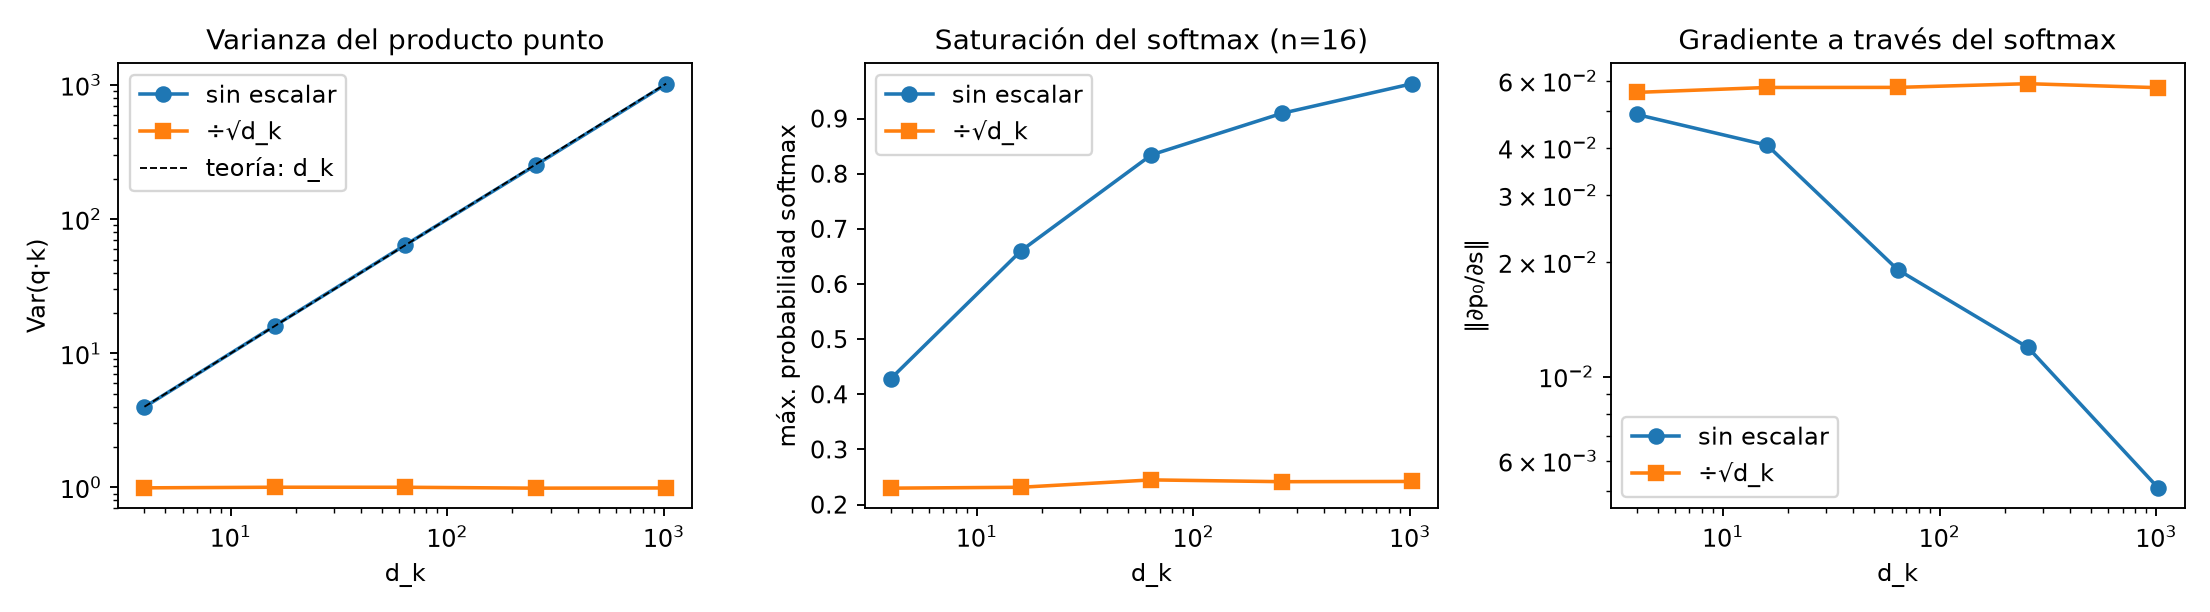
\includegraphics[width=\textwidth]{figs/escalamiento.png}
\caption{Efecto del escalamiento por $\sqrt{\dk}$: varianza del producto punto, saturación del softmax y gradiente.}\label{fig:esc}
\end{figure}
\begin{figure}[h]
\centering
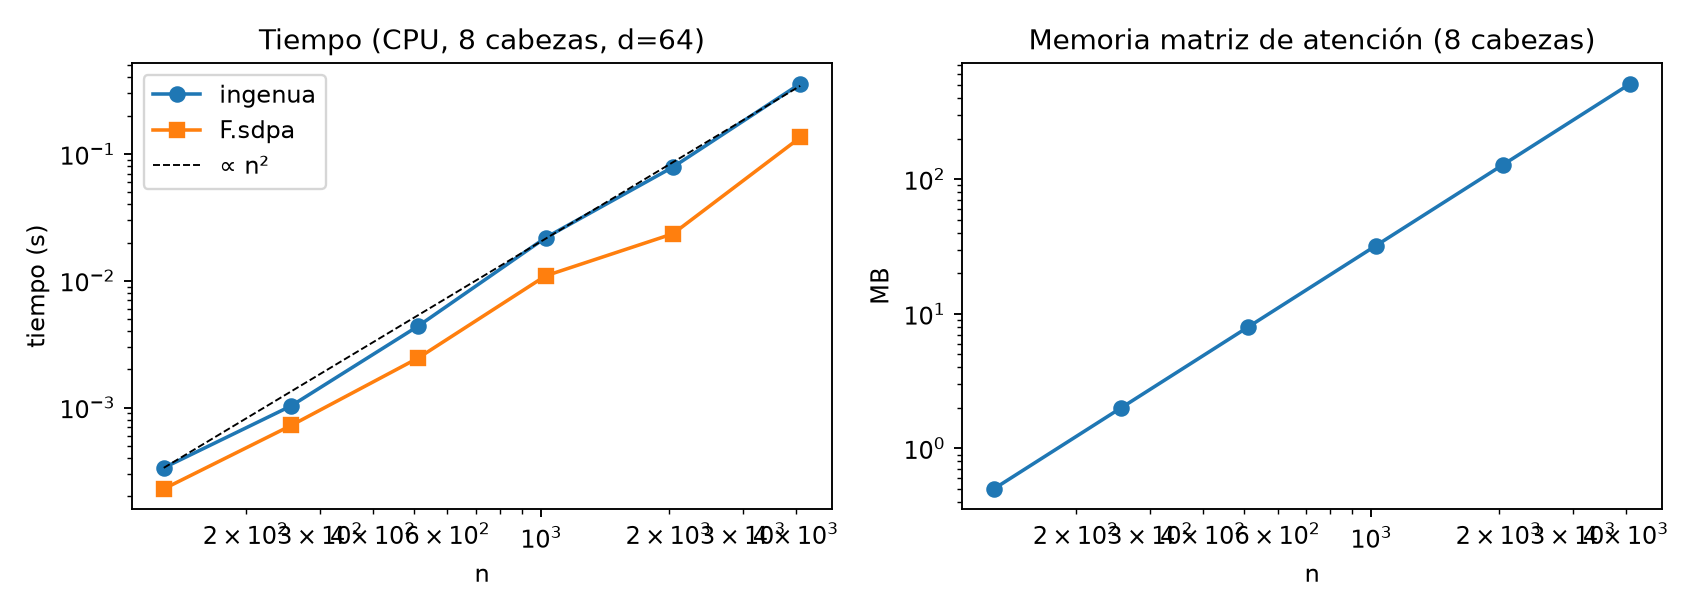
\includegraphics[width=0.78\textwidth]{figs/costo.png}
\caption{Tiempo medido y memoria de la matriz de atención en función de $n$.}\label{fig:costo}
\end{figure}

\section{Mapas de atención e interpretación}
Oración: «The animal didn't cross the street because it was too tired.» (BERT \texttt{bert-base-uncased}, 12 capas $\times$ 12 cabezas; GPT-2 \texttt{gpt2}).

\begin{figure}[h]
\centering
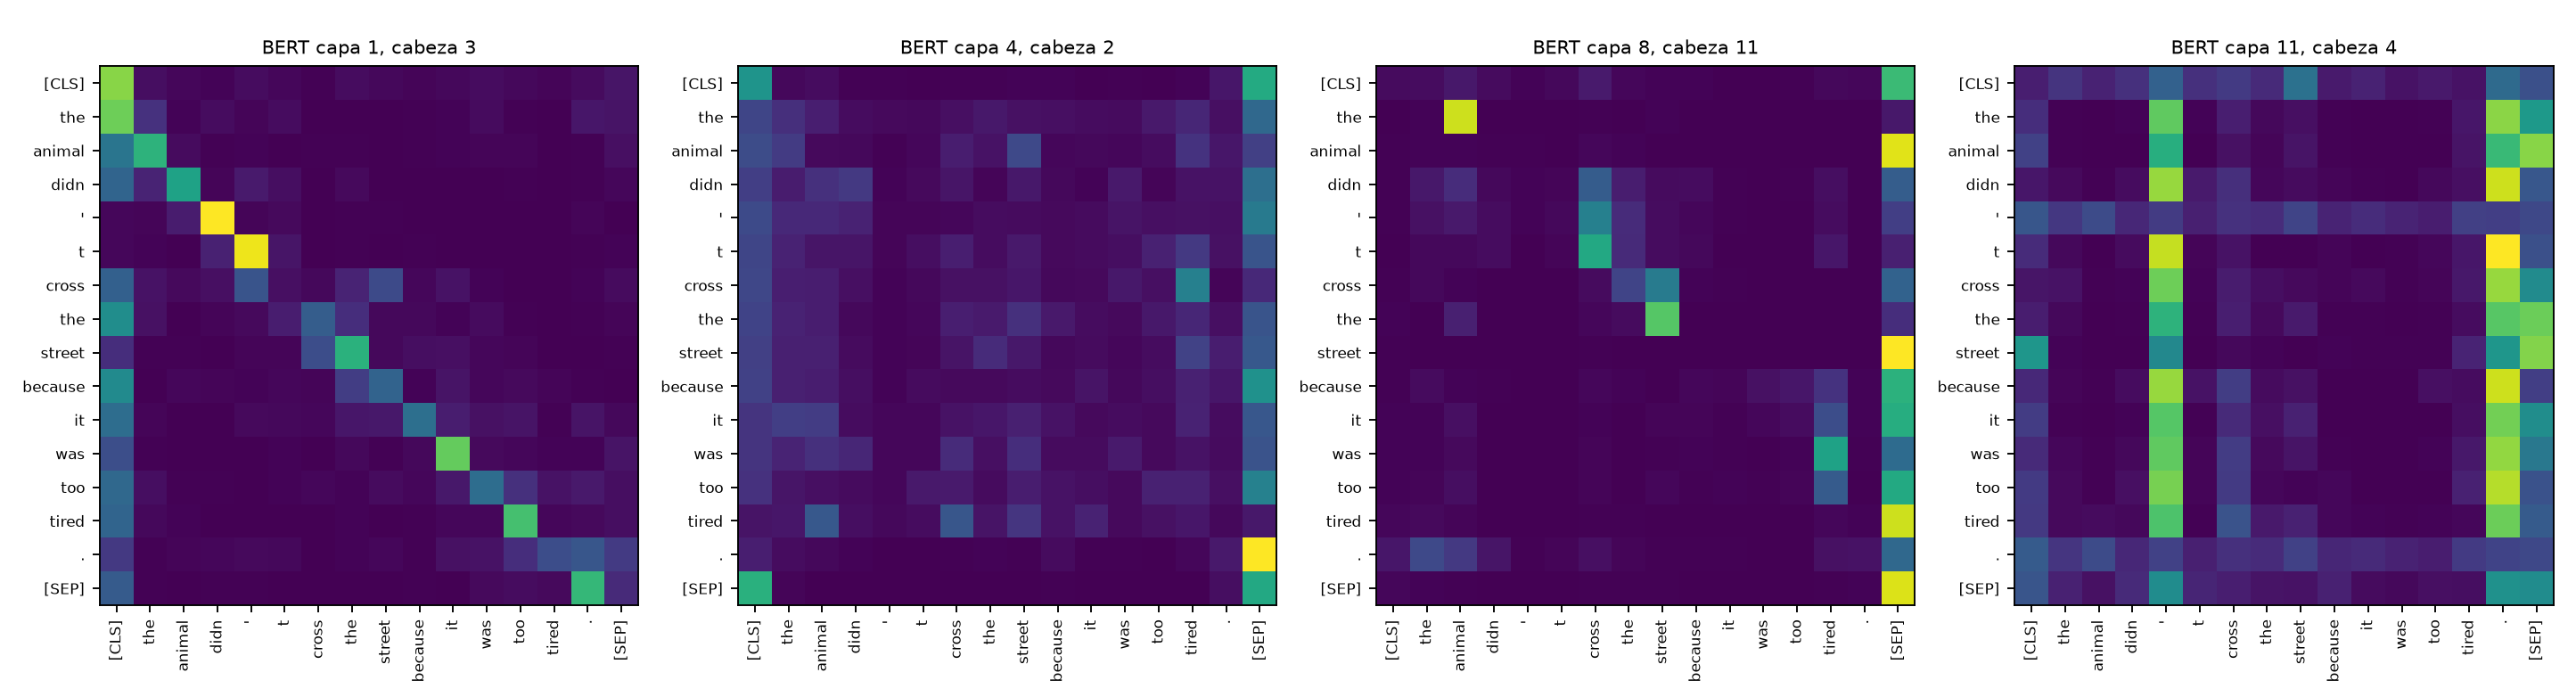
\includegraphics[width=\textwidth]{figs/bert_heads.png}
\caption{Cuatro cabezas de BERT en capas distintas (filas = query, columnas = key).}\label{fig:heads}
\end{figure}

\textbf{Patrones (Fig.~\ref{fig:heads}).} La capa 1, cabeza 3 atiende sobre todo a la propia palabra y al token anterior/[CLS] (patrón posicional local). La capa 4, cabeza 2 y la capa 8, cabeza 11 envían gran parte de la atención a [SEP] y [CLS], y la capa 11, cabeza 4 a la puntuación («'», «.») y [SEP]; estos tokens funcionan como «reposo» cuando no hay información útil que mover. Midiendo las 144 cabezas de BERT, el patrón «token siguiente» llega a 0.95 de la masa de atención (capa 3, cabeza 10), «token anterior» a 0.64 (capa 4, cabeza 6) y [CLS]/[SEP] concentran en promedio 35\,\% de toda la atención.

\begin{figure}[h]
\centering
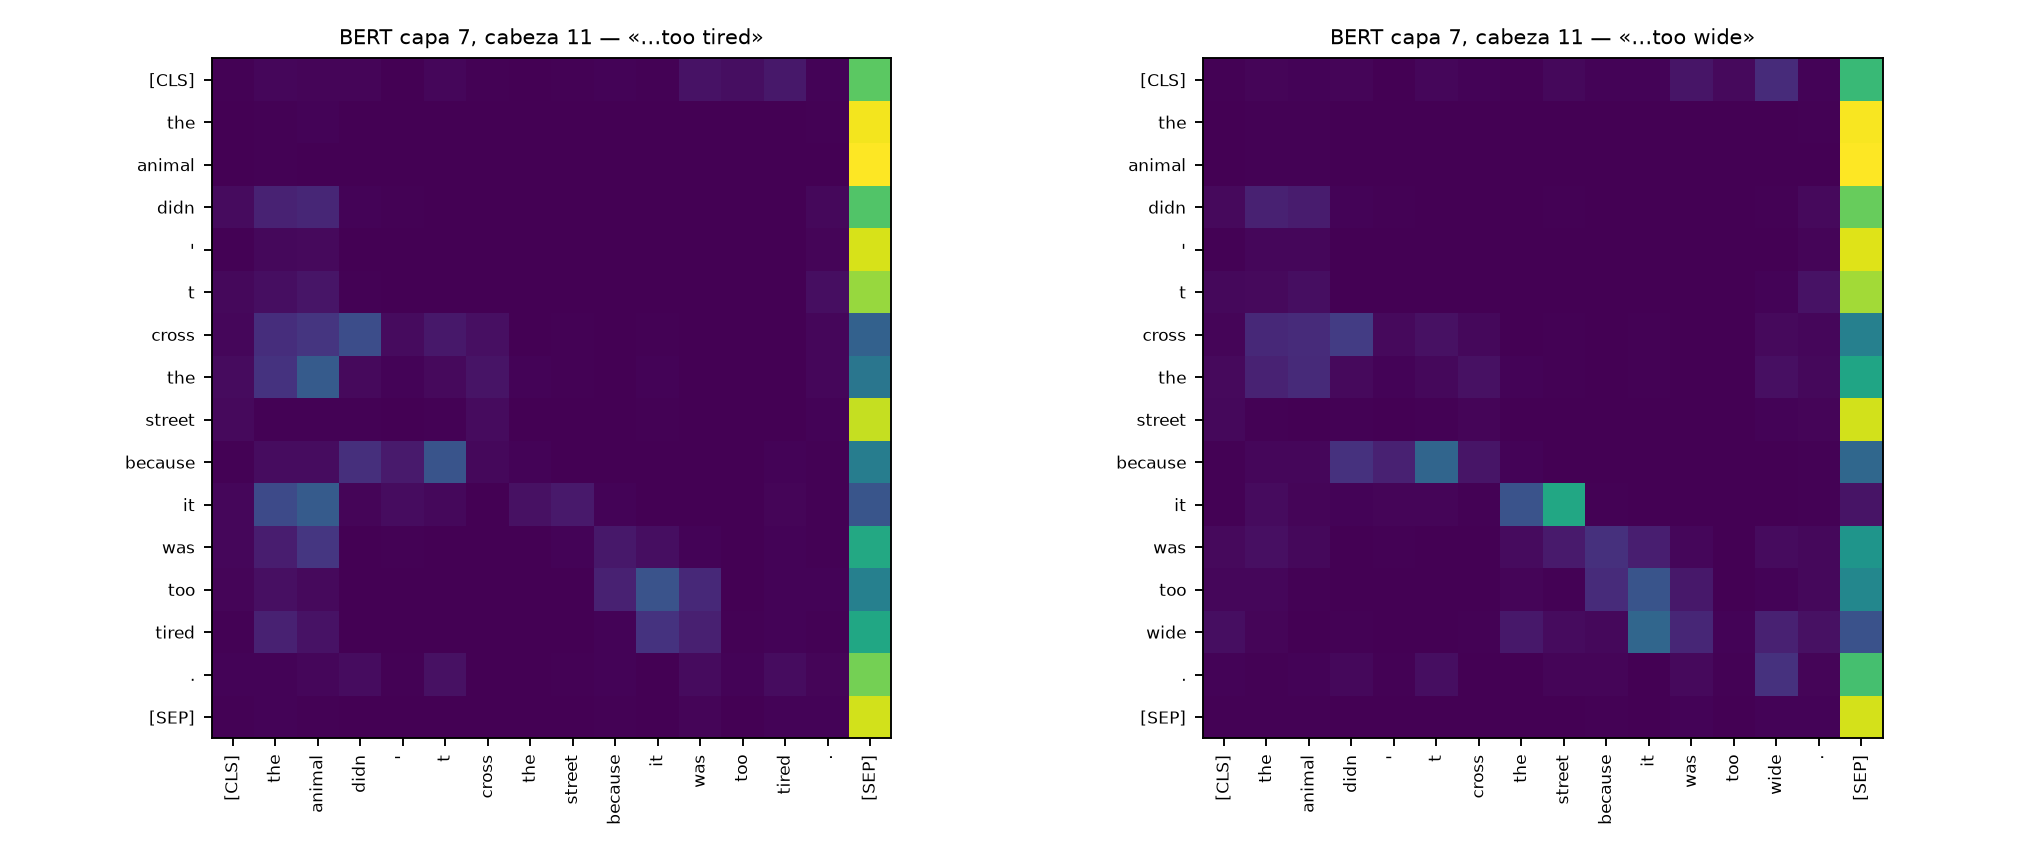
\includegraphics[width=0.78\textwidth]{figs/bert_it.png}
\caption{BERT, capa 7, cabeza 11: atención de «it» con «tired» (izq.) y «wide» (der.).}\label{fig:it}
\end{figure}

\textbf{«it» $\to$ «animal» / «street».} Se buscó, sobre las 144 cabezas, la que más invierte la preferencia entre ambas oraciones. La capa 7, cabeza 11 (Fig.~\ref{fig:it}) es la mejor: con «tired», «it» da 0.284 a «animal» y 0.067 a «street»; con «wide», 0.012 a «animal» y 0.590 a «street». Es decir, la cabeza cambia el referente según el adjetivo, pero es un efecto aislado: otras cabezas (capas 9--11) favorecen siempre «animal» (p.\,ej.\ 0.68 vs.\ 0.00 en «tired» y 0.31 vs.\ 0.26 en «wide»), por lo que no hay una cabeza que «resuelva la correferencia» de forma robusta.

\begin{figure}[h]
\centering
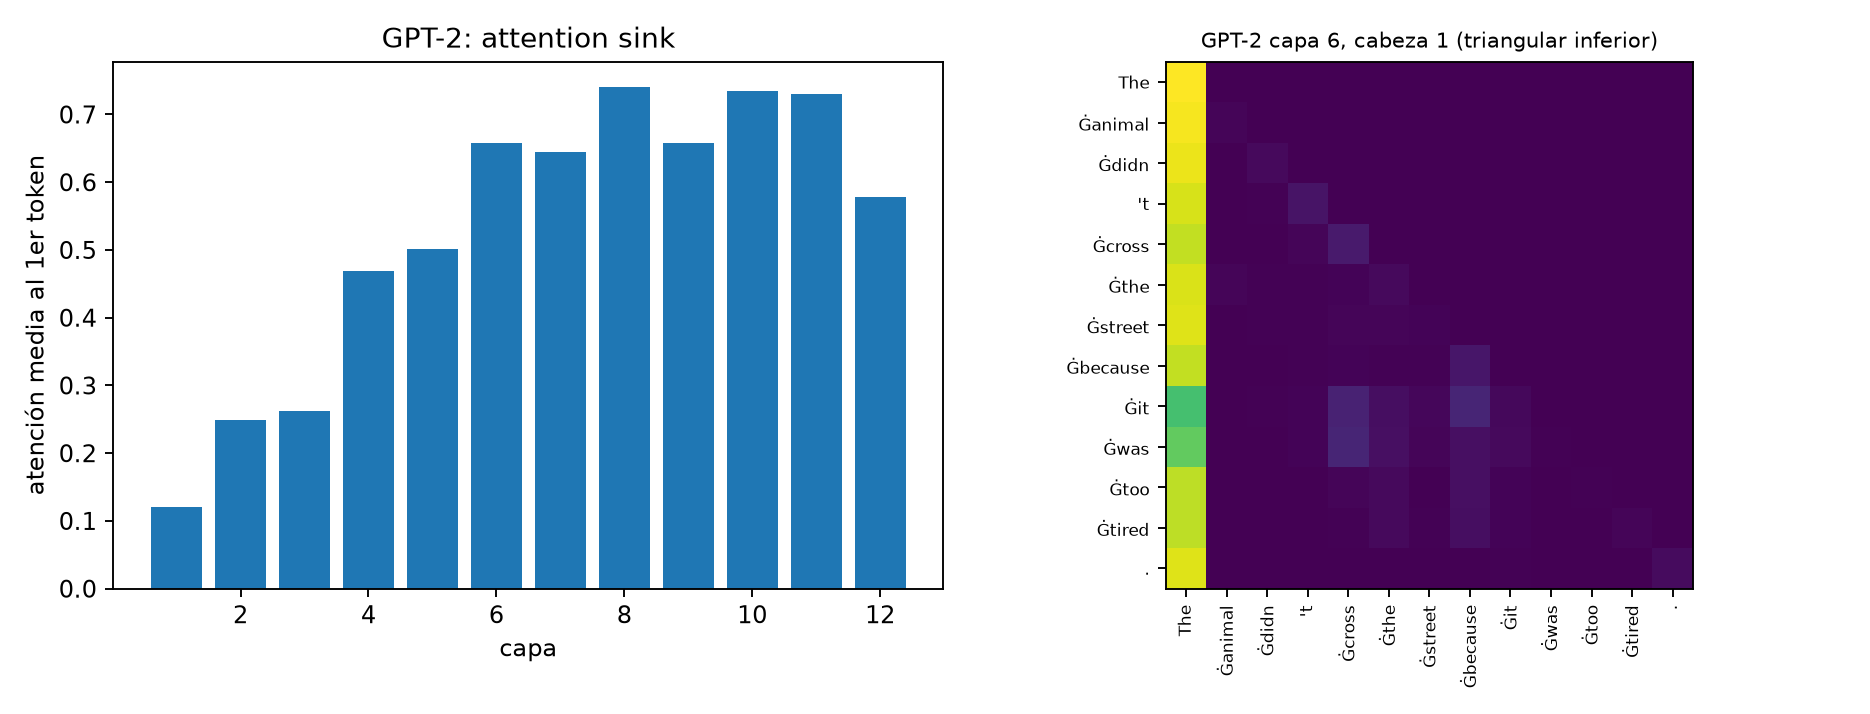
\includegraphics[width=\textwidth]{figs/gpt2_sink.png}
\caption{GPT-2: atención media al primer token por capa y mapa de la capa 6, cabeza 1.}\label{fig:sink}
\end{figure}

\textbf{GPT-2.} Sobre las 12 capas y 12 cabezas la máxima atención hacia posiciones futuras es exactamente 0, es decir, las matrices son triangulares inferiores. Excluyendo la primera fila (donde es trivialmente 1), el primer token recibe en promedio 12\,\% de la atención en la capa 1, 47\,\% en la 4 y hasta 74\,\% en la capa 8 (53\,\% promedio global, Fig.~\ref{fig:sink}). Es el fenómeno de \emph{attention sink} de Xiao et al.\ (2023): como el softmax obliga a repartir masa 1, el modelo deposita la atención «sobrante» en los primeros tokens (visibles para todos), que sirven de ancla y cuyos valores aportan poco.

\begin{figure}[h]
\centering
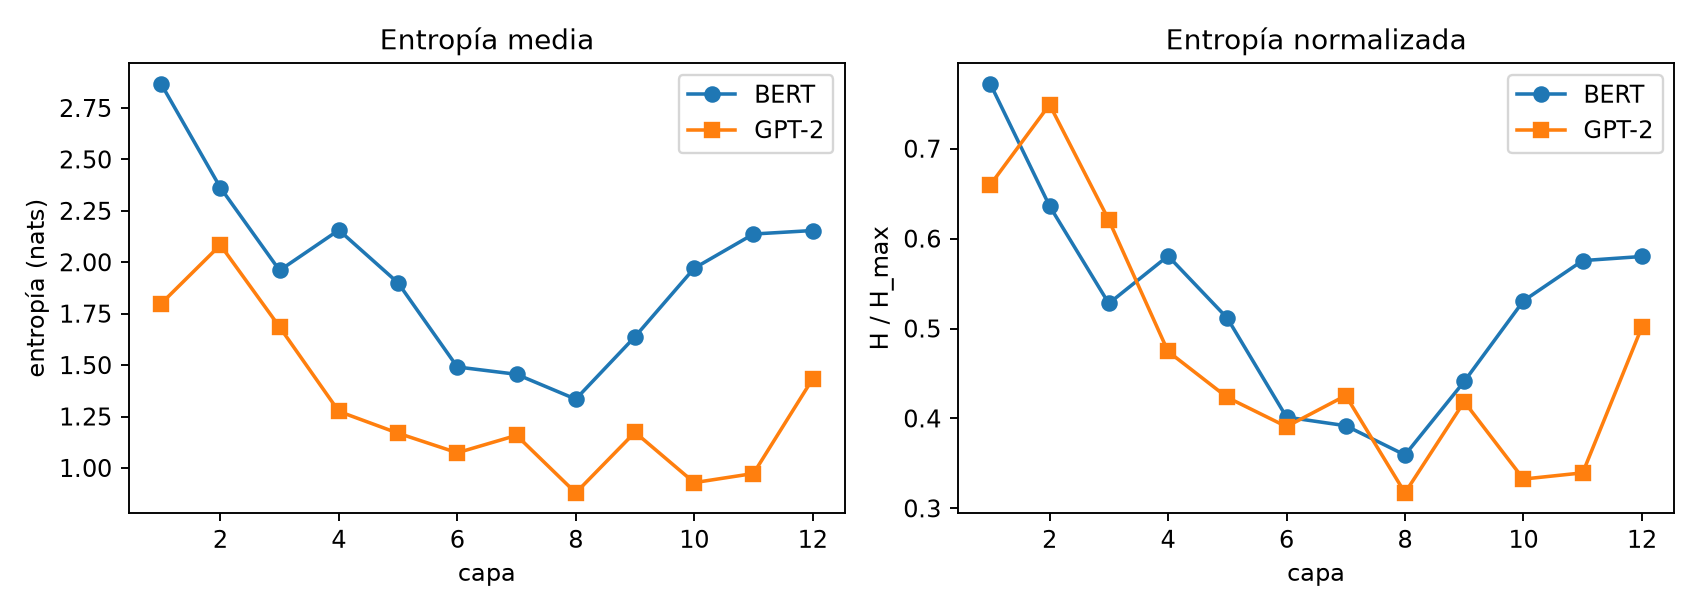
\includegraphics[width=0.78\textwidth]{figs/entropia.png}
\caption{Entropía de Shannon media de la atención por capa (izq.) y normalizada por $\log$ del número de llaves visibles (der.). Texto de 2 oraciones.}\label{fig:ent}
\end{figure}

\textbf{Entropía (Fig.~\ref{fig:ent}).} En ambos modelos la curva no es monótona: es alta en las primeras capas (BERT 2.87 nats, GPT-2 1.80), mínima en las capas intermedias (BERT 1.33 y GPT-2 0.88 en la capa 8) y sube de nuevo al final (BERT 2.15, GPT-2 1.43). Por tanto, las capas profundas \emph{no} atienden de forma más difusa que las intermedias: son más concentradas que las primeras, y la capa 8 es la más puntual. GPT-2 tiene menor entropía absoluta (en parte porque cada query ve menos llaves, pero también tras normalizar queda por debajo de BERT en casi todas las capas profundas, coherente con su sink).

\section{Discusión y análisis}
\textbf{¿Por qué la atención permitió modelos más grandes?} (1) Paralelismo: todas las posiciones de una capa se calculan con multiplicaciones de matrices simultáneas, aprovechando GPU/TPU, mientras que la RNN es secuencial en el tiempo. (2) Longitud de camino: dos tokens cualesquiera se conectan en un salto ($O(1)$ vs.\ $O(n)$), lo que facilita aprender dependencias largas y mejora el flujo de gradiente. (3) El costo cuadrático es el precio, pero con $n$ moderado el cómputo es dominado por matmuls densas y escala bien con datos y parámetros (y FlashAttention reduce la memoria), de modo que se compensa con la paralelización.

\textbf{Especialización de cabezas.} Hay evidencia clara: cabezas casi puramente posicionales (siguiente token 0.95, anterior 0.64), cabezas de [CLS]/[SEP] (0.85 en la capa 8, cabeza 7) y una cabeza (capa 7, cabeza 11) sensible al contexto para «it». Sin embargo, no todas parecen útiles: muchas de las cabezas dedican gran parte de su masa a [CLS]/[SEP] (35\,\% promedio), un comportamiento casi de «no operación»; la literatura (p.\,ej.\ Michel et al., 2019) reporta que muchas cabezas pueden podarse con poca pérdida; aquí solo se observó el patrón de atención, no se hizo poda.

\textbf{¿Explican los pesos las decisiones?} Solo parcialmente. A favor: la cabeza 7/11 cambia de «animal» a «street» de forma coherente con el contexto. En contra: gran parte de la masa va a [SEP] o al primer token (sinks), que no son «razones» semánticas, y otras cabezas favorecen «animal» en ambos casos. Jain y Wallace (2019) muestran que se pueden construir distribuciones de atención muy distintas con la misma predicción y que correlacionan poco con la importancia por gradientes; Wiegreffe y Pinter (2019) matizan que depende de qué se llame «explicación» y de la prueba (con adversarios entrenados, la atención sí aporta una explicación plausible, no necesariamente fiel). Nuestras visualizaciones son consistentes con ambas lecturas: son informativas, pero no son una explicación causal.

\textbf{¿RNN/CNN en lugar de Transformer?} Cuando hay pocos datos o poco cómputo, secuencias muy largas en streaming con memoria constante por paso (inferencia en dispositivos pequeños, series temporales online), o cuando el sesgo inductivo local ayuda (CNN en señales/audio/visión con pocos datos, convoluciones 1D para detección local rápida) y cuando el costo $O(n^2)$ es prohibitivo.

\textbf{Documentos de 100\,000 tokens.} La matriz de atención tendría $10^{10}$ entradas por cabeza y capa ($\approx$40 GB en float32 por cabeza y capa si se materializa), imposible sin truncar; el cómputo también crece cuadráticamente y el KV-cache crece linealmente con $n$. Alternativas: FlashAttention (exacta, memoria lineal), atención por ventanas/dispersa (Longformer, BigBird), atención lineal o modelos de espacio de estados (Mamba), \emph{chunking}/recuperación (RAG) y extensión de contexto con RoPE escalada.

\section{Conclusiones}
(i) El factor $1/\sqrt{\dk}$ es necesario: sin él la varianza crece como $\dk$, el softmax se satura (0.96 para $\dk=1024$) y el gradiente cae un orden de magnitud. (ii) Multi-head redistribuye la capacidad sin añadir parámetros (1\,050\,624 en ambos casos). (iii) El costo medido es cuadrático ($4.5\times$ al duplicar $n$). (iv) Las cabezas se especializan (posicionales, sinks, algunas semánticas), la atención se concentra en capas intermedias y GPT-2 muestra un claro \emph{attention sink} (hasta 74\,\%), pero los mapas de atención son evidencia sugerente, no una explicación completa del modelo.

\section*{Referencias}
\begin{itemize}[leftmargin=1em,itemsep=0pt]\footnotesize
\item Vaswani et al.\ (2017). \emph{Attention Is All You Need}. arXiv:1706.03762.
\item Bahdanau, Cho, Bengio (2015). \emph{Neural Machine Translation by Jointly Learning to Align and Translate}. arXiv:1409.0473.
\item Luong, Pham, Manning (2015). \emph{Effective Approaches to Attention-based NMT}. arXiv:1508.04025.
\item Xiao et al.\ (2023). \emph{Efficient Streaming Language Models with Attention Sinks}. arXiv:2309.17453.
\item Jain, Wallace (2019). \emph{Attention is not Explanation}. arXiv:1902.10186.\quad Wiegreffe, Pinter (2019). \emph{Attention is not not Explanation}. arXiv:1908.04626.
\item Michel, Levy, Neubig (2019). \emph{Are Sixteen Heads Really Better than One?} arXiv:1905.10650.\quad Su et al.\ (2021). \emph{RoFormer (RoPE)}. arXiv:2104.09864.\quad Dao et al.\ (2022). \emph{FlashAttention}. arXiv:2205.14135.
\item Documentación de PyTorch (\texttt{torch.nn}, \texttt{F.scaled\_dot\_product\_attention}) y de Hugging Face Transformers.
\item Código y notebook: \url{https://github.com/AngelEsquit/HT2-DL}
\end{itemize}

\end{document}
